\chapter{Numerical Methods}
\section{The Finite Element Method}
The theory presented in this section is inspired by the great work of Langtangen in "Finite Element Method - INF5620 lecture notes" \cite{Langtangen}  \\
Consider the Poisson-equation
\begin{align}
\nabla^2 \mathbf{u} = \mathbf{f} & \quad \text{ in } \Omega \label{Poisson}\\
\mathbf{u} = \mathbf{u_0} & \quad \text{ on } \partial \label{Poisson_D}\Omega_D \\
\pdi{\mathbf{u}}{n} = \mathbf{g} & \quad \text{ on } \partial \Omega_N \label{Poisson_N}
\end{align}
where $\Omega \in \mathbb{R}^d$ is a domain, $ \mathbf{u} = \mathbf{u}(\mathbf{x})$ is an unknown field and $\mathbf{f}$ is a source function. The boundary, $\partial \Omega$ is divided into two parts. $\partial \Omega_D$ for the Dirichlet boundary condition, and $\partial \Omega_N$ for the Neumann condition. 
\\
\\
\subsection{Weak formulation}
\eqref{Poisson} is known as the strong form of the equation. To reformulate the problem and state a weak formulation we multiply \eqref{Poisson} with a test function $\mathbf{v} \in V$, where $V$ is a function space, and integrate over the domain. Weak formulations are important in the sense that differential equations can be transformed into a system of linear equations. In the rest of this text the following notation is used for the inner product of two functions
\begin{align} (\mathbf{u},\mathbf{v})_{\Omega} = \int_{\Omega} \mathbf{u} : \mathbf{v} \mathrm{d}V \end{align}

By multiplying \eqref{Poisson} with a test function, $\mathbf{v}$ and integrating over the domain, the weak form is obtained
\begin{align}
(\nabla^2 \mathbf{u} - \mathbf{f}, \mathbf{v})_\Omega = 0 & \quad \forall \, \mathbf{v} \in V \label{Projection}
\end{align}
or, after integrating by parts \\ \\
\begin{align}
-(\nabla \mathbf{u}, \mathbf{v})_\Omega + (\mathbf{g}, \mathbf{v})_{\partial \Omega_N} = (\mathbf{f},\mathbf{v})_\Omega & \quad \forall \mathbf{v} \in V \label{Weak_form}
\end{align}
\\
The formulation \eqref{Projection} is known as the projection of a function $\mathbf{u} - \mathbf{f}$ onto the function space $V$. In other words, the error is orthogonal to all functions in $V$. 

\subsection{Finite elements}
The next step is to approximate $\mathbf{u}$ with a sum of basisfunctions in a finite-dimensional function space, $V = \text{span}\{\psi_0, \psi_1, ..., \psi_N\}$. Here, $\mathbf{\psi}_i$ represents the basis functions and we search for a solution $\mathbf{u}_h \in V$ such that $\mathbf{u}_h$ can be written as a linear combination of the basis functions. 
The first step in the finite element method consists of dividing the domain into smaller parts
\begin{align*}
\Omega = \Omega_0 \cup \Omega_1 \cup ... \cup \Omega_{N_e}
\end{align*}
where $N_e$ is the number of elements. Each element have a number of nodes within them depending on what type of basis functions to be used. Let's first consider the continuous Galerkin basis functions, $\phi_i$, in a one-dimensional domain. There is exactly one basisfunction for each node located at $x_i$. These basis functions have the property that
\begin{align*}
\phi_i(x_j) = \begin{cases}
				1 \quad \text{ for } i=j \\
				0 \quad \text{ for } i\neq j
		 		\end{cases}
\end{align*}
That is, the basis functions $\phi_i$ are zero on all nodes except at node $i$. Each basis function is constructed by taking the Lagrange-polynomial which is 1 at the given node and 0 on all other nodes within the same element. Note that the basis functions for a node on the boundary of an element will have two Lagrange-polynomials "pieced together" depending on at which element the basis function is considered. For the rest of the domain the basis functions are defined to be 0. \\ \\

\begin{figure}
  \begin{center}
    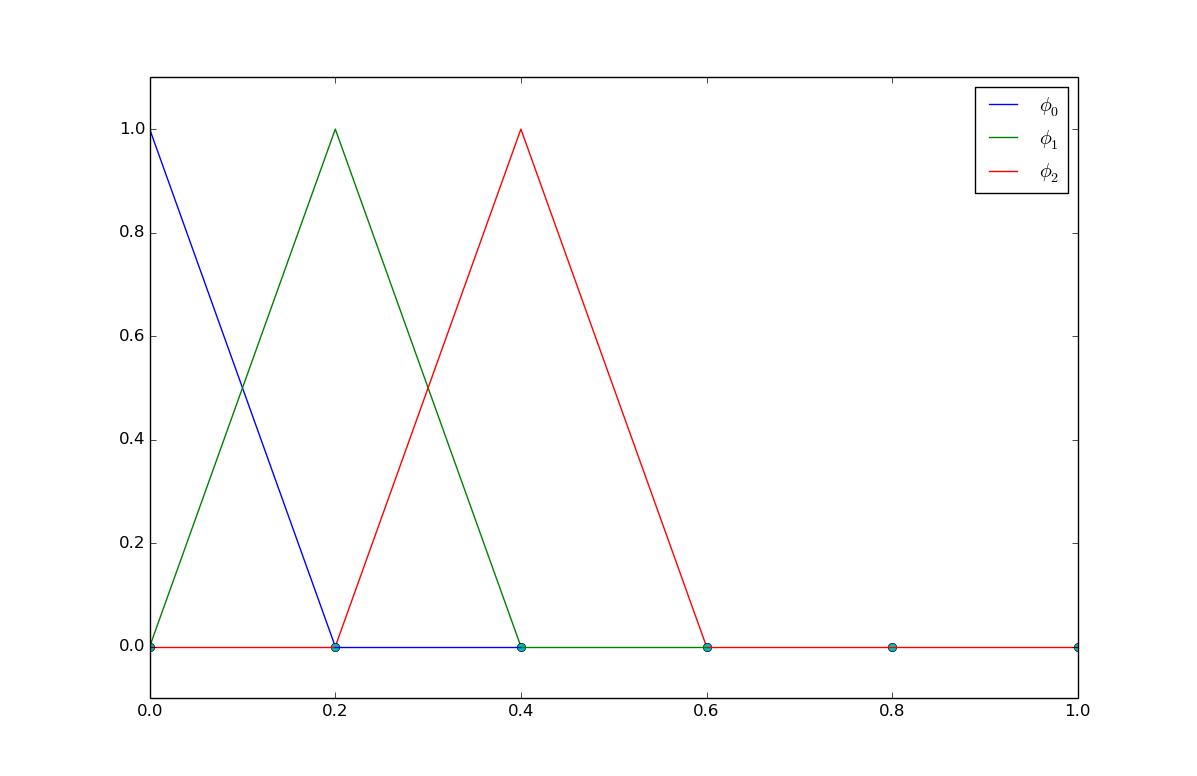
\includegraphics[scale=0.4]{figures/hats.png}
  \end{center}
	\caption{The three first linear basis functions on the unit interval divided uniformly into 5 elements}
\end{figure}
Now, let's return to the original problem \eqref{Poisson}-\eqref{Poisson_N}. We start by approximating u as a linear combination of all the basis functions. 
\begin{align}
u_h = \sum_{i=0}^N c_i \phi_i \label{u_hsum}
\end{align}
The definitions of $u_h$ and $V$ now give rise to a linear system. Using the summation convention $x_i\,y_i = \sum_0^N x_i y_i $, \eqref{Weak_form} is now written 
\begin{align}
-c_i(\nabla \phi_i, \phi_j)_\Omega = (f,\phi_j) - (g, \phi_j)_{\partial \Omega_N} \label{Linear_system}
\end{align}
\\
\\

The right hand side of \eqref{Linear_system} is known as the bilinear form while the left hand side is the linear form, assuming the normal derivative is known on the boundary. In the case of Dirichlet boundary conditions all test functions $\phi_j$ will take the value 0 on $\partial \Omega_D$ and the linear system will be adjusted to take these boundary conditions into account. \\
The system can be written in matrix form, and in the end the problem consists of solving the linear system
\begin{align} A_{i,j}c_i = b_j \label{Matrix_1} \end{align}
\\
\\
\section{Implementation in FEniCS}
When the variational form has been carried out, implementation in FEniCS is relatively simple. We need a computational mesh, appropriate function spaces, a variational form and boundary conditions to have a well-posed problem. 
\\
\section{A Discontinuous Galerkin method}
Discontinuous Galerkin (DG) methods is a relatively new tool for CFD simulations. The method itself was developed during the 1970s and has been used increasingly the last few decades. Unlike with the Continuous Galerkin elements, we now allow the solution to be discontiuous, i.e cells do not share nodes anymore. Instead of solving over the whole domain, we now seek approximate continuous solutions on each cell independently of the others. To this end it is convenient to define the average and jump of a discontinuous variable
\begin{align} 
\{\mathbf{u}\} = \frac{1}{2}(\mathbf{u}^+ + \mathbf{u}^-) \hspace{2 cm}  [\mathbf{u}]  =  \mathbf{u}^+ - \mathbf{u}^- \label{Avg_jump}
\end{align}
where $\mathbf{u}^+$ and $\mathbf{u}^-$ is the solution at two neighboring cells at cell $E^+$ and $E^-$. The normal vectors are denoted $\mathbf{n}^+$ and $\mathbf{n}^-$. If consistent the choice of $\mathbf{n}$ is arbitrary. 
\subsection{Stokes flow}
By integrating Stokes equation by parts, adding symmetry and penalty terms as in \cite{Riviere2005} we end up with a DG-method ready for use. Since the method involves many terms we derive a weak formulation for each term. All sets of facets are denoted as $e$, interior facets as $\Gamma$ and exterior facets as $\partial \Omega$. Starting with the diffusion term $-\mu \nabla ^2 u$, we multiply with a test function and integrate by parts:
\begin{align}
	\mu \sum_{E \in e} (\nabla u, \nabla v)_E 
   -\mu \sum_{E \in \Gamma}([v], \{ \nabla u \} \cdot n_e)_E 
   -\mu \sum_{E \in \Gamma}([u], \{ \nabla v \} \cdot n_e)_E 
	+ \frac{\alpha}{h} \sum_{E \in \Gamma}([u],[v])_E \nonumber \\
	-\mu \sum_{E \in \partial \Omega}(v,  \nabla u \cdot n_e)_E 
   -\mu \sum_{E \in \partial \Omega}(u,  \nabla v  \cdot n_e)_E 
	+ \frac{\beta}{h} \sum_{E \in \partial \Omega}(u,v)_E 
 \label {Diffusion}
\end{align}
Similiarly, the contributions from the term $\nabla p$ will be
\begin{align}
	- \sum_{E \in e}(p, \nabla \cdot v)_E - \sum_{E \in \Gamma}
\end{align}
